
\section{Experimental Study} 
\label{sec:exp}

To test how well the implemented algorithms work we executed the games a lot of times. We have the 20 games from the trainings- and validationset to test the algorithms. We had no acces to the origial test set. First of all we want to compare the 3 different controllers with each other but the several different parameters we can change in the controllers are also interesting.
To test a agent we ran 1000 Games, one game 50 times and one single level 10 times. The following machine was used to run all of the simulations:

\begin{table}
\center
\begin{tabular}{ll} 
\textbf{CPU} & 4x Inted(R) Core(TM) i5-4210U CPU @ 1.70Ghz \\ \hline
\textbf{Memory} & 8 GB DDR3 L \\  \hline
\textbf{Operating System} \mbox{   } & Ubuntu 14.04.1 LTS \\  \hline
\textbf{Java Version} &  1.7.0\_65\\  
\end{tabular}
\caption{experiment setup}
\end{table}


Only this machine was used because with the same agent and parameters we achieved on different machines very different results. The computational power from the CPU was decisive for our choice. The reason of the different results is that the agent every game tick only has 40 ms to return an action. The results from a powerful CPU were better and more stable (the derivation was lower) than the results from an worse CPU. To evaluate the results we stored them in csv files and generated tables.

For every evaluation is first of all a table with all there parameter settings. Additionally there are the average winning rate and the standard deviation listed.
All the results are also visualized by boxplots. There you can see the minimum and maximum average wins overall iterations. Furthermore the blue rectangle shows 
the qartile values. The red line in the middle is the median and the blue dot is the mean (average wins).
Do not mix quartiles with the standard deviation that is something completely different.
In the following sections each of the approaches is evaluated. 


\subsection{Heuristic based Algorithm} 

The heuristic based algorithm has several parameter that changes the behaviour of the agent (cf.~\cref{tbl:heur}).
Firstly we just changed the maximal states field that provides a limit for saved states at
the A* algorithm. As you can see the average winning rate increases by changing to a higher maximal states limit up to 20.
But if the variable is set to 25 we had a worse result. This might be that if this value is to low the target is not found 
by the A* algorithm. Moreover if it is to large to many states are saved and we get trouble with the memory or the
garbage collector.


\begin{table}[htbp]
\center
\begin{tabular}{*9c}  \hline
\multicolumn{1}{p{1cm}}{\centering ID} & 
\multicolumn{1}{p{2cm}}{\centering Max.\\ States} & 
\multicolumn{1}{p{2cm}}{\centering Safety\\ Strategy} & 
\multicolumn{1}{p{2cm}}{\centering Safety\\ Iterations} & 
\multicolumn{1}{p{1cm}}{\centering Avg\\ Wins	} & 
\multicolumn{1}{p{1cm}}{\centering Std of Wins} \\ \hline
1 & 5 & SafetyAdvance & 5 & 0.517 & 0.026 \\ \hline
2 & 15 & SafetyAdvance & 5 & 0.529 & 0.020\\ \hline
\textbf{3} & \textbf{20} & \textbf{SafetyAdvance} & \textbf{5} & \textbf{0.532} & \textbf{0.027} \\ \hline
4 & 25 & SafetyAdvance & 5 & 0.521 & 0.019 \\ \hline
5 & 20 & SafetyGridSearch & - & 0.498 & 0.024 \\ \hline
6 & 20 & SafetyIntelligent & 5 & 0.527 & 0.018 \\ \hline
\end{tabular}
\caption{results of the \ac{HR} algorithms}
\label{tbl:heur}
\end{table}
\vspace{-2cm}
\begin{figure}[H]
\centering
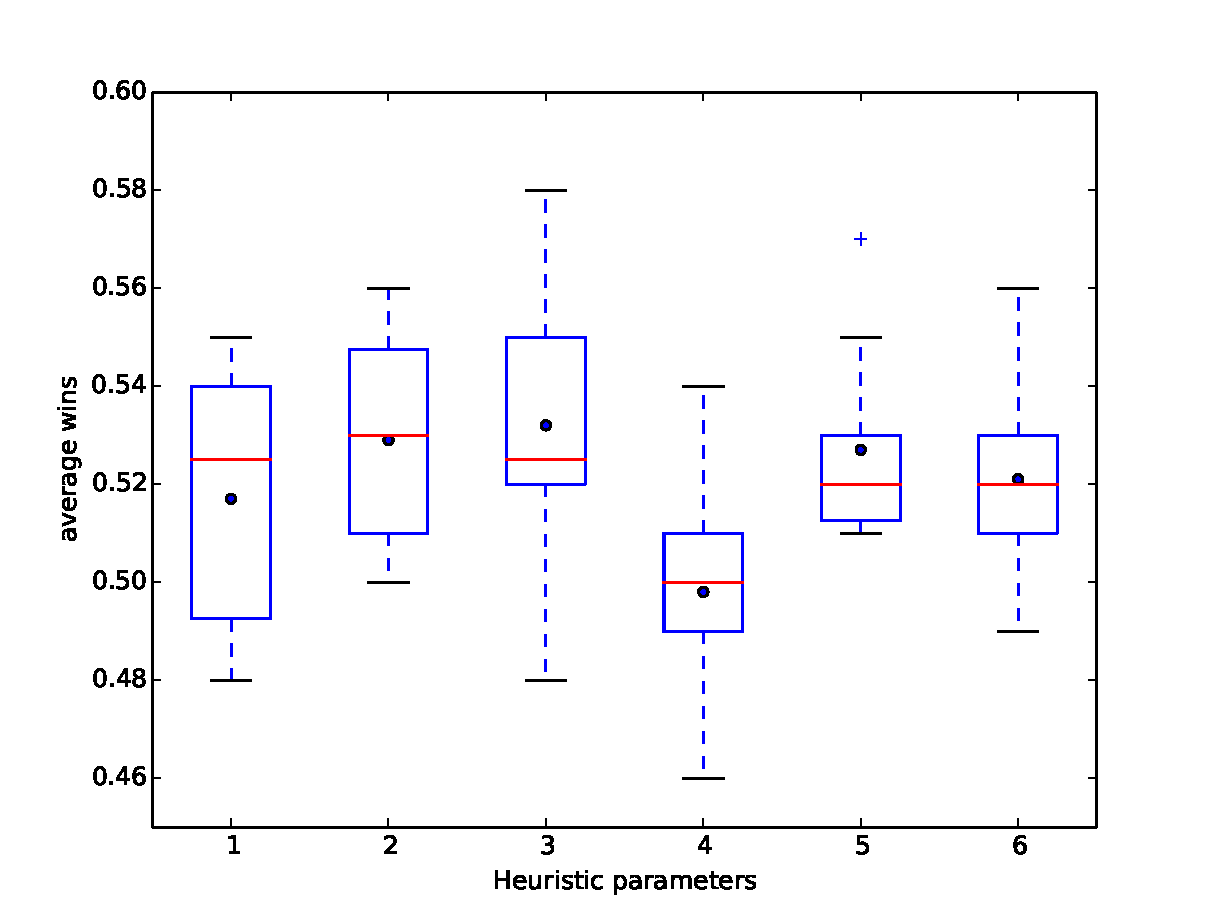
\includegraphics[scale=0.5]{images/eval_heur.pdf}
\caption{boxplot of the heuristic based algorithms}
\label{fig:eval_heur}
\end{figure}

After that we tried to change the safety strategy to the grid and the intelligent search. Both results
are worse than the SafetyAdvance Strategy. Since the SafeGridSearch highly depends on the Explorer and the
classification of the object this might be the cause.
With the SafetyIntelligent we got no further improvement but it is nearly good as the SafetyAdvance approach.

The boxplot (cf.~\cref{fig:eval_heur}) visualizes the quartiles. The best parameter setup has also the largest
quartile range. When you look at the table also the largest standard deviation (which doesn't have to be the same).
If the target is not found the agent is staying alive. The risk of a longer search to reach a simulation state
that collides with the target could be the reason for the higher variance of the results.



\subsection{MCTS} 

For the test of the \ac{MCTS} algorithm we modified three different parameter. First of all we try to figure out
if the rolling horizon idea makes sense. After that we changed the gamma variable that is used
as a \textit{discounting factor}. Since there we no further improvement the discounting was disabled by setting it to 1.
As a third and very important variable we experimented with the maximal tree depth. Due to the fact that we are using an open loop approach this determines 
the size of the tree with recommended actions.


\begin{minipage}{1\textwidth}
\begin{table}[H]
\center
\begin{tabular}{*9c}  \hline
\multicolumn{1}{p{1cm}}{\centering ID} & 
\multicolumn{1}{p{2cm}}{\centering rolling \\ Horizon} & 
\multicolumn{1}{p{2cm}}{\centering maximal \\ TreeDepth} & 
\multicolumn{1}{p{1.5cm}}{\centering gamma} & 
\multicolumn{1}{p{2cm}}{\centering Avg\\ Wins	} & 
\multicolumn{1}{p{2cm}}{\centering Std of Wins} \\ \hline
1 & 0 & 10 & 1 & 0.383 & 0.033 \\ \hline
2 & 1 & 10 & 0.9 & 0.401 & 0.026 \\ \hline
3 & 1 & 3 & 1 & 0.416 & 0.014\\ \hline
4 & 1 & 5 & 1 & 0.402 & 0.030 \\ \hline
\textbf{5} & \textbf{1} & \textbf{7} & \textbf{1} & \textbf{0.422} & \textbf{0.033} \\ \hline
6 & 1 & 10 & 1 & 0.412 & 0.025 \\ \hline
7 & 1 & 15 & 1 & 0.394 & 0.014\\ \hline
8 & 1 & 20 & 1 & 0.395 & 0.025 \\ \hline
9 & 1 & 25 & 1 & 0.384 & 0.026 \\ \hline
\end{tabular}
\caption{\ac{MCTS} result}
\label{mcts_result}
\end{table}
\vspace{-2cm}
\begin{figure}[H]
\centering
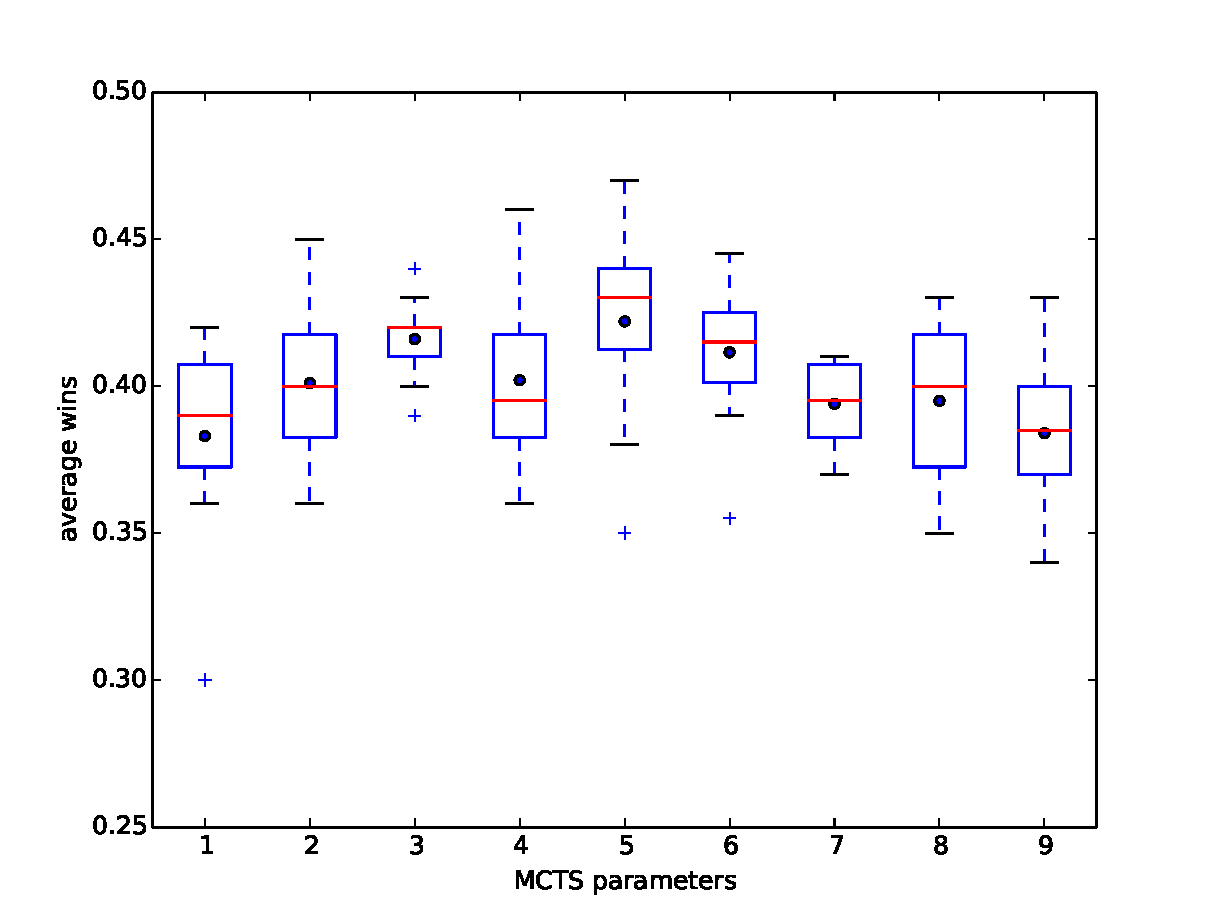
\includegraphics[scale=0.6]{images/eval_mcts.pdf}
\caption{boxplot of the \ac{MCTS} algorithm}
\label{fig:eval_evo}
\end{figure}
\end{minipage}

We reached the best result by using an agent with rolling horizon, a maximal tree depth of 7 
and no discounted reward (cf.~\cref{mcts_result}). 
A higher maximal tree depth sticks together with a depth first search. Therefore the winning rate
becomes lower at some value. If the tree is to small (e.g. hight of one) it's really a breadth-first search.

We also tried to combine several approaches for example using the heuristic explorer 
for a better \ac{MCTS} iteration. But that idea is difficult to implement because this
it's a trade off of exploration, exploitation and heuristic search needed. Since that is
not easy to handle a first naive ideas brought worse results, we got not manage it to evaluate 
this combination of two approaches.
It might be one future work to try and implement that.



\subsection{Evolutionary Algorithm} 

For the \ac{EA} algorithm exists many parameters that could be modified. To find a
good setup we created an evolutionary algorithm over that parameter of the \ac{EA}
algorithm. This meta-evolution uses the winning rate as a score function and
varies the different parameters. Since we need more computational power to
get really good result we were not able to use that idea. Instead we defined
the different agents (cf.~\cref{ea_result}).

As a first parameter we modified the \textit{SafetyIterations} which ensure that the agent do not
choose an action that causes death.
Furthermore the path length of each individual and the size of the pool were changed.
Since not all candidates are shifted to the next generation we introduced a variable
that manages that quantity. At least we evaluated if our dynamic path length what
ensures the achievement of a specific generation makes sense.


\begin{table}[H]
\center
\begin{tabular}{*9c}  \hline
\multicolumn{1}{p{1cm}}{\centering ID} & 
\multicolumn{1}{p{2cm}}{\centering Safety\\ Iterations} & 
\multicolumn{1}{p{1cm}}{\centering Path Length} & 
\multicolumn{1}{p{1cm}}{\centering Size of\\ Pop.} & 
\multicolumn{1}{p{1cm}}{\centering Fittest\\ Pop.} & 
\multicolumn{1}{p{1cm}}{\centering Dyn. Path\\ Length} & 
\multicolumn{1}{p{1cm}}{\centering Min. Gen.} & 
\multicolumn{1}{p{1cm}}{\centering Avg \\ Wins	} & 
\multicolumn{1}{p{1cm}}{\centering Std of Wins} \\ \hline
1 & 2 & 6 & 14 & 5 & no & - & 0.459 & 0.023 \\ \hline
2 & 4 & 6 & 10 & 4 & no & - & 0.458 & 0.024 \\ \hline
3 & 5 & 4 & 14 & 5 & no & - & 0.466 & 0.028 \\ \hline
4 & 5 & 6 & 10 & 5 & no & - & 0.459 & 0.032 \\ \hline
5 & 5 & 6 & 13 & 4 & yes & 5 & 0.451 & 0.041 \\ \hline
6 & 5 & 6 & 14 & 3 & no & - & 0.471 & 0.018 \\ \hline
7 & 5 & 6 & 14 & 5 & no & - & 0.461 & 0.025 \\ \hline
\textbf{8} & \textbf{5} & \textbf{6} & \textbf{14} & \textbf{5} & \textbf{yes} & \textbf{2} & \textbf{0.479} & 0.021 \\ \hline
9 & 5 & 6 & 14 & 5 & yes & 4 & 0.463 & 0.027 \\ \hline
10 & 5 & 6 & 14 & 5 & yes & 6 & 0.449 & 0.041 \\ \hline
11 & 5 & 6 & 14 & 7 & no & - & 0.474 & 0.028 \\ \hline
12 & 5 & 6 & 18 & 5 & no & - & 0.462 & 0.035 \\ \hline
13 & 5 & 8 & 14 & 5 & no & - & 0.453 & 0.029 \\ \hline
14 & 8 & 6 & 14 & 5 & no & - & 0.477 & 0.022 \\ \hline
\end{tabular}
\caption{results of the \ac{EA} algorithms}
\label{ea_result}
\end{table}


\begin{figure}[H]
\centering
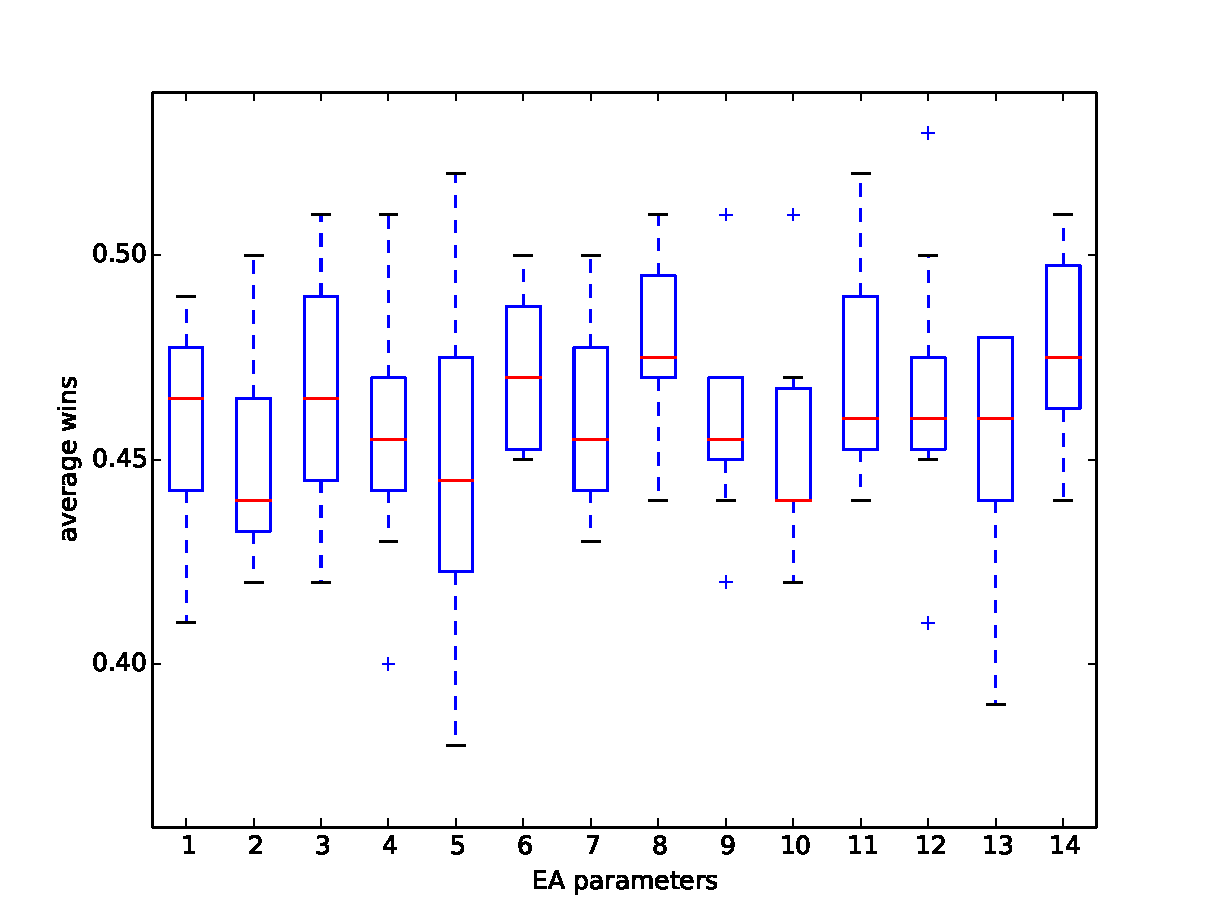
\includegraphics[scale=0.6]{images/eval_evolutionary.pdf}
\caption{boxplot of the \ac{EA} algorithms}
\label{fig:eval_evo}
\end{figure}

As you can see (cf.~\cref{fig:eval_evo}) the \ac{EA} approach has a higher
interquartile range than the others.
We assume this is caused by the idea of \acp{EA} that the randomness is very important.
In average we reached the best result with the parameters of \textit{ID} 8 (cf.~\cref{ea_result}). 
Since another agent 14 with no dynamic path length reached also a very good result this idea might
not help for winning the games. This is assured by the best one that only has a min generation value 
of 2 what should normally for all agents be the case. Otherwise it's only a random approach.




\subsection{Evaluation of all approaches} 

Finally we compare the best parameter setups of the three approaches. We defined the best as the agent with the highest average winning rate.
The selected agents are printed bold at each of the result tables.
For a complete comparison there are also the average score and the played time steps evaluated.
The highest winning rate is reached by the heuristic controller (cf.~\cref{tbl:all_result}).
But for the highest score we can see that the \ac{MCTS} approaches reaches more points than the others.
For that we can suppose, that the \ac{HR} is playing tighter than the other. This is supported by the least played time steps as well.
Playing tight leads to an earlier win. But there are some games where we could first of all collect points and increase the score and
win at the end.


\begin{table}[H]
\center
\begin{tabular}{*9c}  \hline
\multicolumn{1}{p{1cm}}{\centering approach} & 
\multicolumn{1}{p{1.5cm}}{\centering Avg \\ Wins	} & 
\multicolumn{1}{p{1.5cm}}{\centering Std \\ Wins} &
\multicolumn{1}{p{1.5cm}}{\centering Avg \\ Score	} & 
\multicolumn{1}{p{1.5cm}}{\centering Std \\ Score} &
\multicolumn{1}{p{1.5cm}}{\centering Avg \\ timesteps	} & 
\multicolumn{1}{p{1.5cm}}{\centering Std \\ timesteps} \\ \hline
HR & \textbf{0.527} & 0.029 & 165.05 & 59.51 & \textbf{695.86} & 36.17 \\ \hline
MCTS & 0.467 & 0.034 & \textbf{230.69} & 74.64 & 942.06 & \textbf{34.00} \\ \hline
EA & 0.470 & \textbf{0.026} & 178.33 & \textbf{51.85} & 818.72 & 38.47 \\ \hline
\end{tabular}
\caption{results of all algorithms}
\label{tbl:all_result}
\end{table}

By looking at the boxplot of the winning rate (cf.~\cref{fig:eval_all_wins})

\todo{adjust the pictures}

\begin{figure}
\begin{minipage}{7cm}
\centering
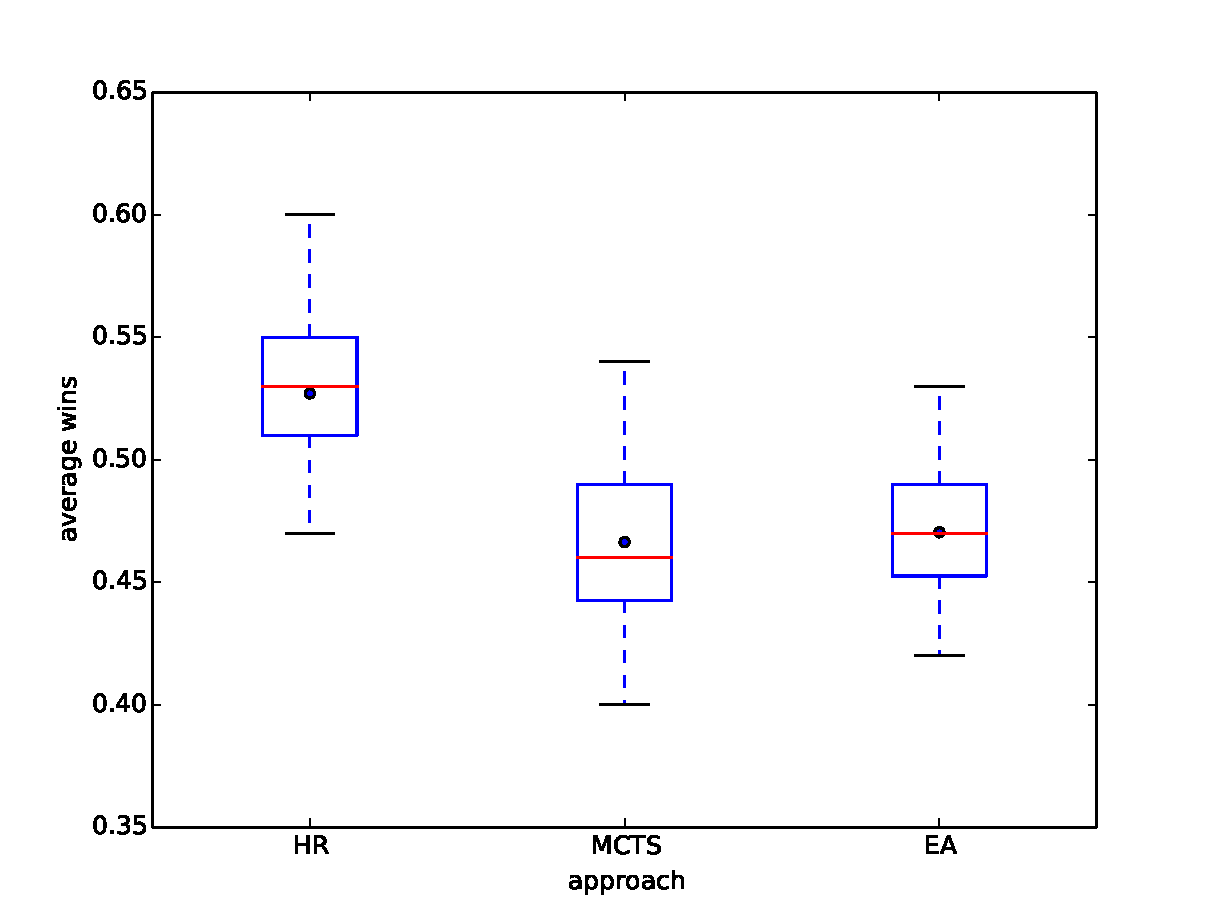
\includegraphics[scale=0.3]{images/eval_all_wins.pdf}
\caption{boxplot of wins}
\label{fig:eval_all_wins}
\end{minipage}%
\begin{minipage}{5cm}
\centering
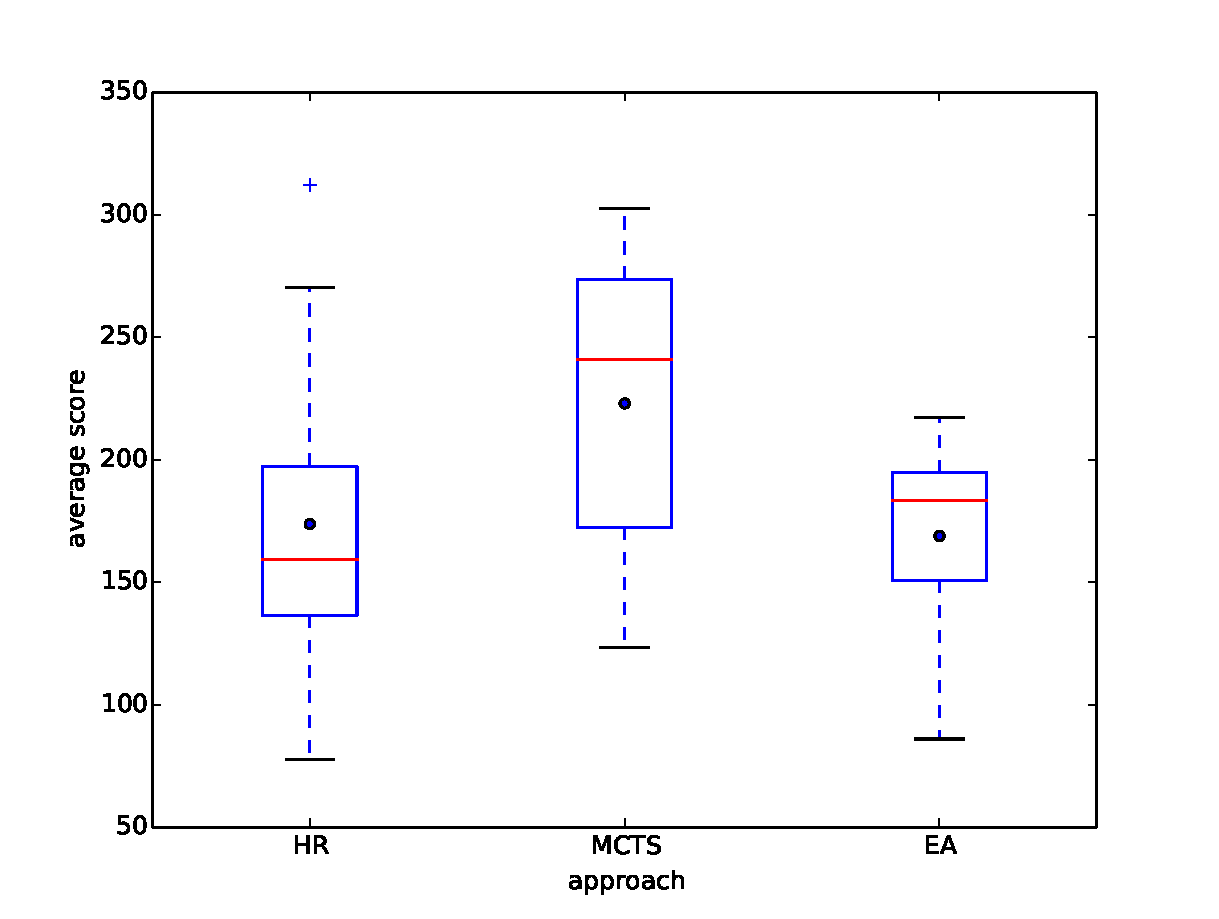
\includegraphics[scale=0.3]{images/eval_all_score.pdf}
\caption{boxplot of score}
\label{fig:eval_all_score}
\end{minipage}
\begin{minipage}{1\textwidth}
\centering
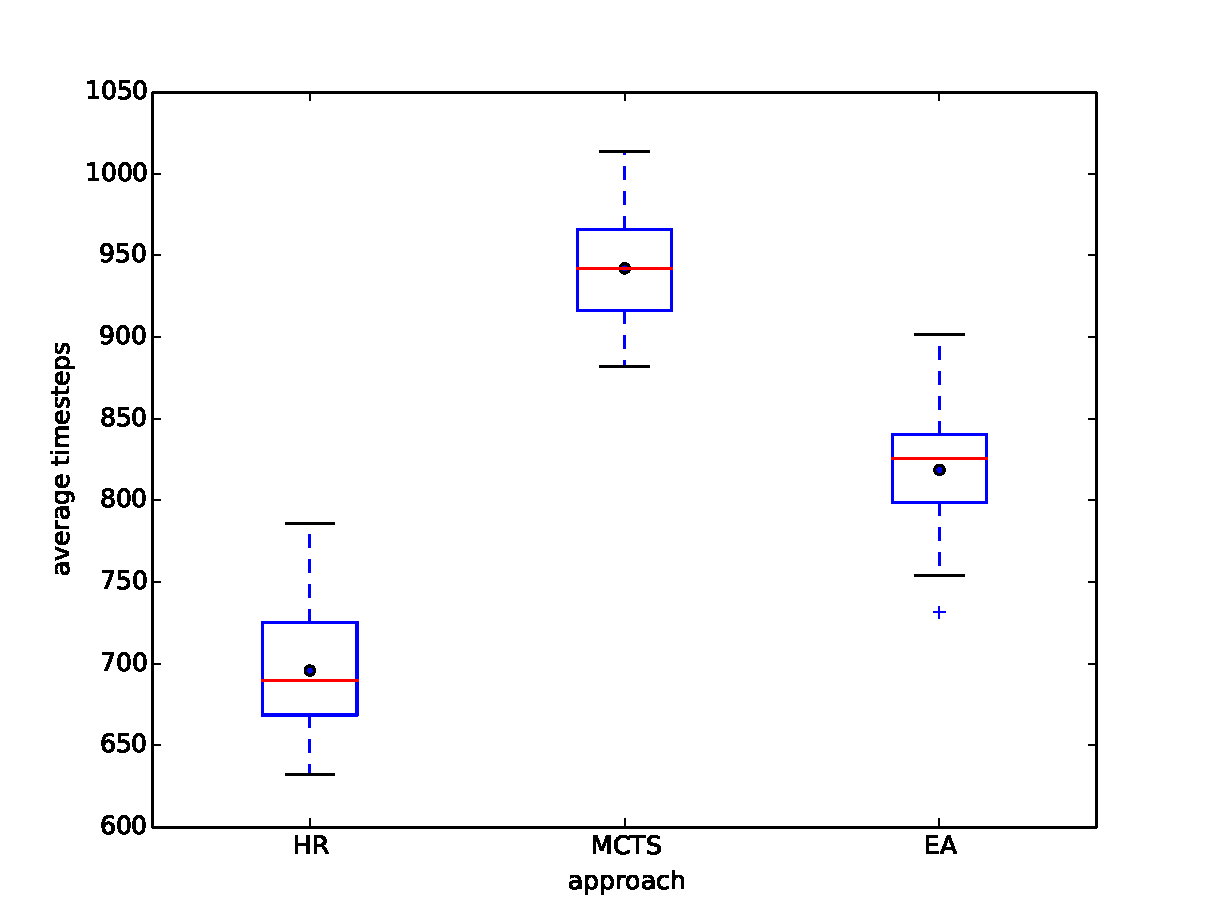
\includegraphics[scale=0.35]{images/eval_all_timesteps.pdf}
\caption{boxplot of timesteps}
\label{fig:eval_all_timesteps}
\end{minipage}
\end{figure}
